\documentclass[12pt]{report}

\usepackage[utf8]{inputenc}
\usepackage[french]{babel}
\usepackage{fullpage}
\usepackage{graphicx}
\usepackage{fancyhdr}	% headers/footers
\usepackage{xcolor}		% to use our own color
\usepackage{lastpage}	% to easily know the total number of pages
\usepackage{titling}	% to easily know the total number of pages
\usepackage{colortbl}	% to put color in a table background
\usepackage{datetime}	% to allow us set a new date formatting
\usepackage{multirow}   % to allow multirows in tables
\usepackage[colorlinks,linkcolor=black]{hyperref}
%% \usepackage[colorlinks=false, urlcolor=blue, breaklinks, pagebackref, citebordercolor={0 0 0}, filebordercolor={0 0 0}, linkbordercolor={0 0 0}, pagebordercolor={0 0 0},
%%                      runbordercolor={0 0 0}, urlbordercolor={0 0 0}, pdfborder={0 0 0}]{hyperref}

% Custom defines zone

% Define useful hand-made colors
\definecolor{epiBlue}{RGB}{23,54,93}
\definecolor{lightGray}{gray}{0.85}

% Bit of code to bold an entire table row
% http://tex.stackexchange.com/questions/4811/make-first-row-of-table-all-bold
\newcolumntype{$}{>{\global\let\currentrowstyle\relax}}
\newcolumntype{^}{>{\currentrowstyle}}
\newcommand{\rowstyle}[1]{\gdef\currentrowstyle{#1}%
  #1\ignorespaces
}

% Defining a "dd/mm/yyyy" date format
\newdateformat{dashDate}{\twodigit{\THEDAY}/\twodigit{\THEMONTH}/\twodigit{\THEYEAR}}

% Define Document Title
\newcommand{\ProjectTitle}{[2015][Onitu]}
\newcommand{\DocTitle}{Gantt}
\newcommand{\LongDocTitle}{Diagramme de Gantt et WBS}

% Setting the space between each page's header and its content
\setlength{\headsep}{0.2in}

% end of Defines


% fancyhdr-specific commands
\setlength{\headheight}{15.2pt}

%% Defining headers and footers contents.

% Big dirty hack of the "empty" pagestyle to show header and footer on the title page (in wait of a better solution)
\fancypagestyle{empty}
{
	\renewcommand{\headrulewidth}{0pt}
	\renewcommand{\footrulewidth}{1pt}
	\fancyhead[L]{
\includegraphics[height=42pt]{logo_eip.png}
	}
	\fancyhead[R]{\colorbox{epiBlue}{\color{white}\textbf{\Large{\ProjectTitle[\DocTitle]} } }
	}

	\fancyfoot[L]{
   		\textcolor{gray}{\{EPITECH.\}}
	}
	\fancyfoot[C]{
		\jobname
	}
	\fancyfoot[R]{}
}

\fancypagestyle{EIP}
{
	\renewcommand{\headrulewidth}{0pt}
	\renewcommand{\footrulewidth}{1pt}
	\fancyhead[L]{
\includegraphics[height=42pt]{logo_eip.png}
	}
	\fancyhead[R]{\colorbox{epiBlue}{\color{white}\textbf{\Large{\ProjectTitle[\DocTitle]} } }
	}

	\fancyfoot[L]{
   		\textcolor{gray}{\{EPITECH.\}}
	}
	\fancyfoot[C]{
		\jobname
	}
	\fancyfoot[R]{
		\thepage/\pageref{LastPage}
	}
}

\pagestyle{EIP} % does not seem to work ...

% end of fancyhdr stuff

%Gummi|063|=)

%\title{The Title\\\normalsize A Sub-title}
\title{
	\huge{\textbf{\textcolor{epiBlue}{EIP Onitu} } }\\
	\Large{\textbf{\emph{\textcolor{gray}{\LongDocTitle} } } }
}


\begin{document}
\addtocontents{toc}{\protect\refstepcounter{page}} % makes the table of contents count pages from 1 (one)
\maketitle

\thispagestyle{empty}
\vspace*{10mm}

\textbf{\emph{\textcolor{onitu}{\large{Résumé du document} } } }\\

Résumé !!!

\clearpage


\thispagestyle{empty}
\vspace*{10mm}
\textbf{\emph{\textcolor{epiBlue}{Description du document} } }\\

\begin{tabular}{|>{\columncolor[gray]{0.85}\color{epiBlue} \bfseries } l|l|}
\hline
	Titre & \LongDocTitle\\
\hline
	Date & \dashDate\today \\
\hline
	Auteur & Alexandre BARON\\
\hline
	Responsable & Louis Roché\\
\hline
	E-Mail & onitu\_2015@labeip.epitech.eu\\
\hline
	Sujet & \LongDocTitle\\
\hline
	Mots clés & Gantt, WBS\\
\hline
	Version du modèle & 1.0\\
\hline
\end{tabular}
\vspace*{10mm}

\textbf{\emph{\textcolor{epiBlue}{Tableau des révisions} } }\\


\begin{tabular}{|$l|p{4cm}|p{2cm}|p{5cm}|}
\hline
\rowcolor{lightGray}
\rowstyle{ \color{epiBlue} \bfseries}
	Date & Auteur & Section(s) & Commentaires\\
\hline
	10/04/2013 & Alexandre Baron & Toutes & Nouveau template \\
\hline
	11/04/2013 & Wannes Rombouts & Contexte & Ajout de la section \\
\hline
	12/04/2013 & Antoine Rozo & Jalons & Ajout de la section \\
\hline
	& & & \\
\hline
\end{tabular}

\tableofcontents
\addtocontents{toc}{\protect\thispagestyle{empty}
                    \protect\pagestyle{empty}}
\thispagestyle{empty}

\chapter{Rappel de l'EIP}
\thispagestyle{EIP} % seems mandatory
\setcounter{page}{1} %reset the page count

\section{Qu'est-ce qu'un EIP et Epitech}
Epitech, école d'expertise informatique en cinq ans, offre aux étudiants l'opportunité de réaliser un projet de fin d'études sur trois ans, l'EIP (pour \emph{Epitech Innovative Project}).\\

À ce titre, les élèves doivent s'organiser en un groupe d'au moins cinq personnes et choisir un sujet porteur de nouveautés ou améliorant un ancien sujet. L'EIP est un passage obligatoire et unique dans la scolarité de l'étudiant, de par son envergure (18 mois) et la préparation requise. Le but est, à la fin du temps imparti, d'obtenir un projet commercialisable.


\section{Principe de base du système futur}
    Onitu est un projet visant à proposer une implémentation libre et Open Source du serveur d’Ubuntu One.\\

    Ubuntu One est un service de Canonical (sponsor officiel d'Ubuntu) permettant de disposer d’un espace de stockage en ligne qui sera synchronisé entre différents ordinateurs et périphériques compatibles via un logiciel client. Le client et le protocole d’Ubuntu One sont disponibles sous licence libre. Néanmoins, le serveur est propriétaire et n’a pas été publié.\\

    L'objectif d'Onitu de proposer un équivalent libre à ce serveur, afin de profiter des fonctionnalités d’Ubuntu One tout en maîtrisant le stockage des données et des informations.\\

    Les fichiers gérés par Onitu pourront être stockés sur un serveur administré par un utilisateur, ou bien sur des services tiers comme Dropbox, Amazon S3, ou Google Drive.\\

    La cible première d'Onitu est l'utilisateur averti, soucieux des problématiques de centralisation des données, et son entourage, à qui il fera profiter le serveur mis en place. Il n'est pas forcément technicien mais assez curieux, le profil même de l'utilisateur Ubuntu.
    Onitu vise aussi à être utilisé au sein d'entreprises ayant la volonté de maîtriser facilement le stockage de leur données.\\


\chapter{Contexte}
\section{Risques}
Notre projet étant dans le domaine du cloud qui est très à la mode ces dernieres années, et qui voit naitre de nouvelles solutions régulierement, il y'as un risque qu'une solution équivalent concurente plus avancée voit le jour, mais nous suposons pour l'instant que ce ne sera pas le cas.

\section{Hypothèses}
Nous suposons que les developpeurs travaillant déjà sur les diférents systèmes par lesquels notre projet est concerné sont ouvert et disposé a nous aiguiller. D'après nos premiers échanges, nous suposons aussi qu'ils ne sont pas hostile a notre implémentation open-source.

Nous avons l'intention de ne développer qu'un serveur et donc de nous reposer sur des clients ubuntu-one déjà existants pour nos tests. Ces clients devront très probablement être modifiés legerement de facon a pouvoir les faire fonctionner avec d'autres serveurs que ceux de canonical. Nous esperont que ces modification seront simple et bien recu par leur auteurs respectifs.

Nous ésperont pouvoir nous organiser de facon de facon éfficace durant la quatrieme année en fesant des groupres de travail par fuseau horaire ce qui devrasis augmenter notre productivité et tout de meme permettre une bonne avancée de projet durant l'année a venir.

\section{Contraintes}
Le projet étant opensource nous devrons respecter certaines contraintes imposés par les licenses choisis. Celle-ci doivent elle mêmes encore être étudier et determiner.

L'architecture complete du projet devra être fixer avant Juin 2013 pour pouvoir être presenter durant la Soutenance avec le LabEIP.

Une des contraintes principales de notre projet sera inhérente au dévelopement de celui-ci. En effet il faudra tenir compte du besoin de modification des clients et de l'implementation d'au moins certaines interfaces de stockage (par exemple le stockage local) avant de pouvoir réelement essayer nos idées dans des conditions réeles.

Nous devrons aussi être capable d'organiser des réunions régulieres, et ce malgrès le décalage horraire.

Enfin, du à l'eloigenement géographique il sera plus compliquer de maintenir une platforme de test pour notre solution d'hebergement. Nous seront probablement ammené a prendre un serveur dédiée de test accesible de nos diférentes destinations en tek4.


\thispagestyle{EIP}

\chapter{Planification}
\thispagestyle{EIP}
\section{Jalons principaux du projet et lotissement}
\subsection{Jalons du planning EIP Epitech}
Cet ensemble de jalons est commun à tous les groupes, car imposé par le planning EIP.


Une première famille de jalons est formée par les bilans d'architecture AA1 et AA2, respectivement du 20 juin et 1er septembre 2013. Ces jalons devront donc mettre terme aux choix et possibilités au niveau de l'architecture du projet.

Une seconde concerne les bilans techniques, et bilans techniques finaux, répartis de façon régulière de novembre 2013 à janvier 2015. Ils s'axeront avec des jalons propres à notre projet et devront marquer des tournants décisifs, tels que des finalisations de lots.


Enfin, la troisième rassemble les deux soutenances finales, de 4ème année en septembre 2014, et de 5ème en février 2015. Ils représenteront pour leur part des livraisons de versions avancée pour la première, et finale pour la seconde.


\subsection{Jalons propres au projet Onitu}
Ces jalons sont définis au niveau de notre projet et marquent donc des points importants de celui-ci. Ils sont à mettre en parallèle avec l'ensemble précédent, dans le sens où ces derniers représentaient des dates importantes, pour lesquelles ces points devront être atteints.


Tout d'abord, il sera nécessaire de posséder un client minimal de test, pour permettre le développement du serveur, tout en continuant celui du client.


Ensuite, l'obtention d'un serveur fonctionnel, puis d'un serveur complet et fonctionnel marqueront deux étapes très importantes du projet.


Les derniers jalons concernent les clients, et correspondent à la finalisation du fork du client officiel, et de la webUI.


\subsection{Définition du lotissement}
Notre lotissement est formé des différentes parties du projet, à savoir: le fork du client officiel Ubuntu One (ajoutant le choix du serveur à utiliser), la webUI (interface complète de gestion avec partage de fichiers), le serveur (conception et réalisation des API, de la base de données), et les drivers (Donnant accès à des ressources internes comme externes pour le stockage des données).

\newpage

\section{WBS}
\begin{figure}[ht]
    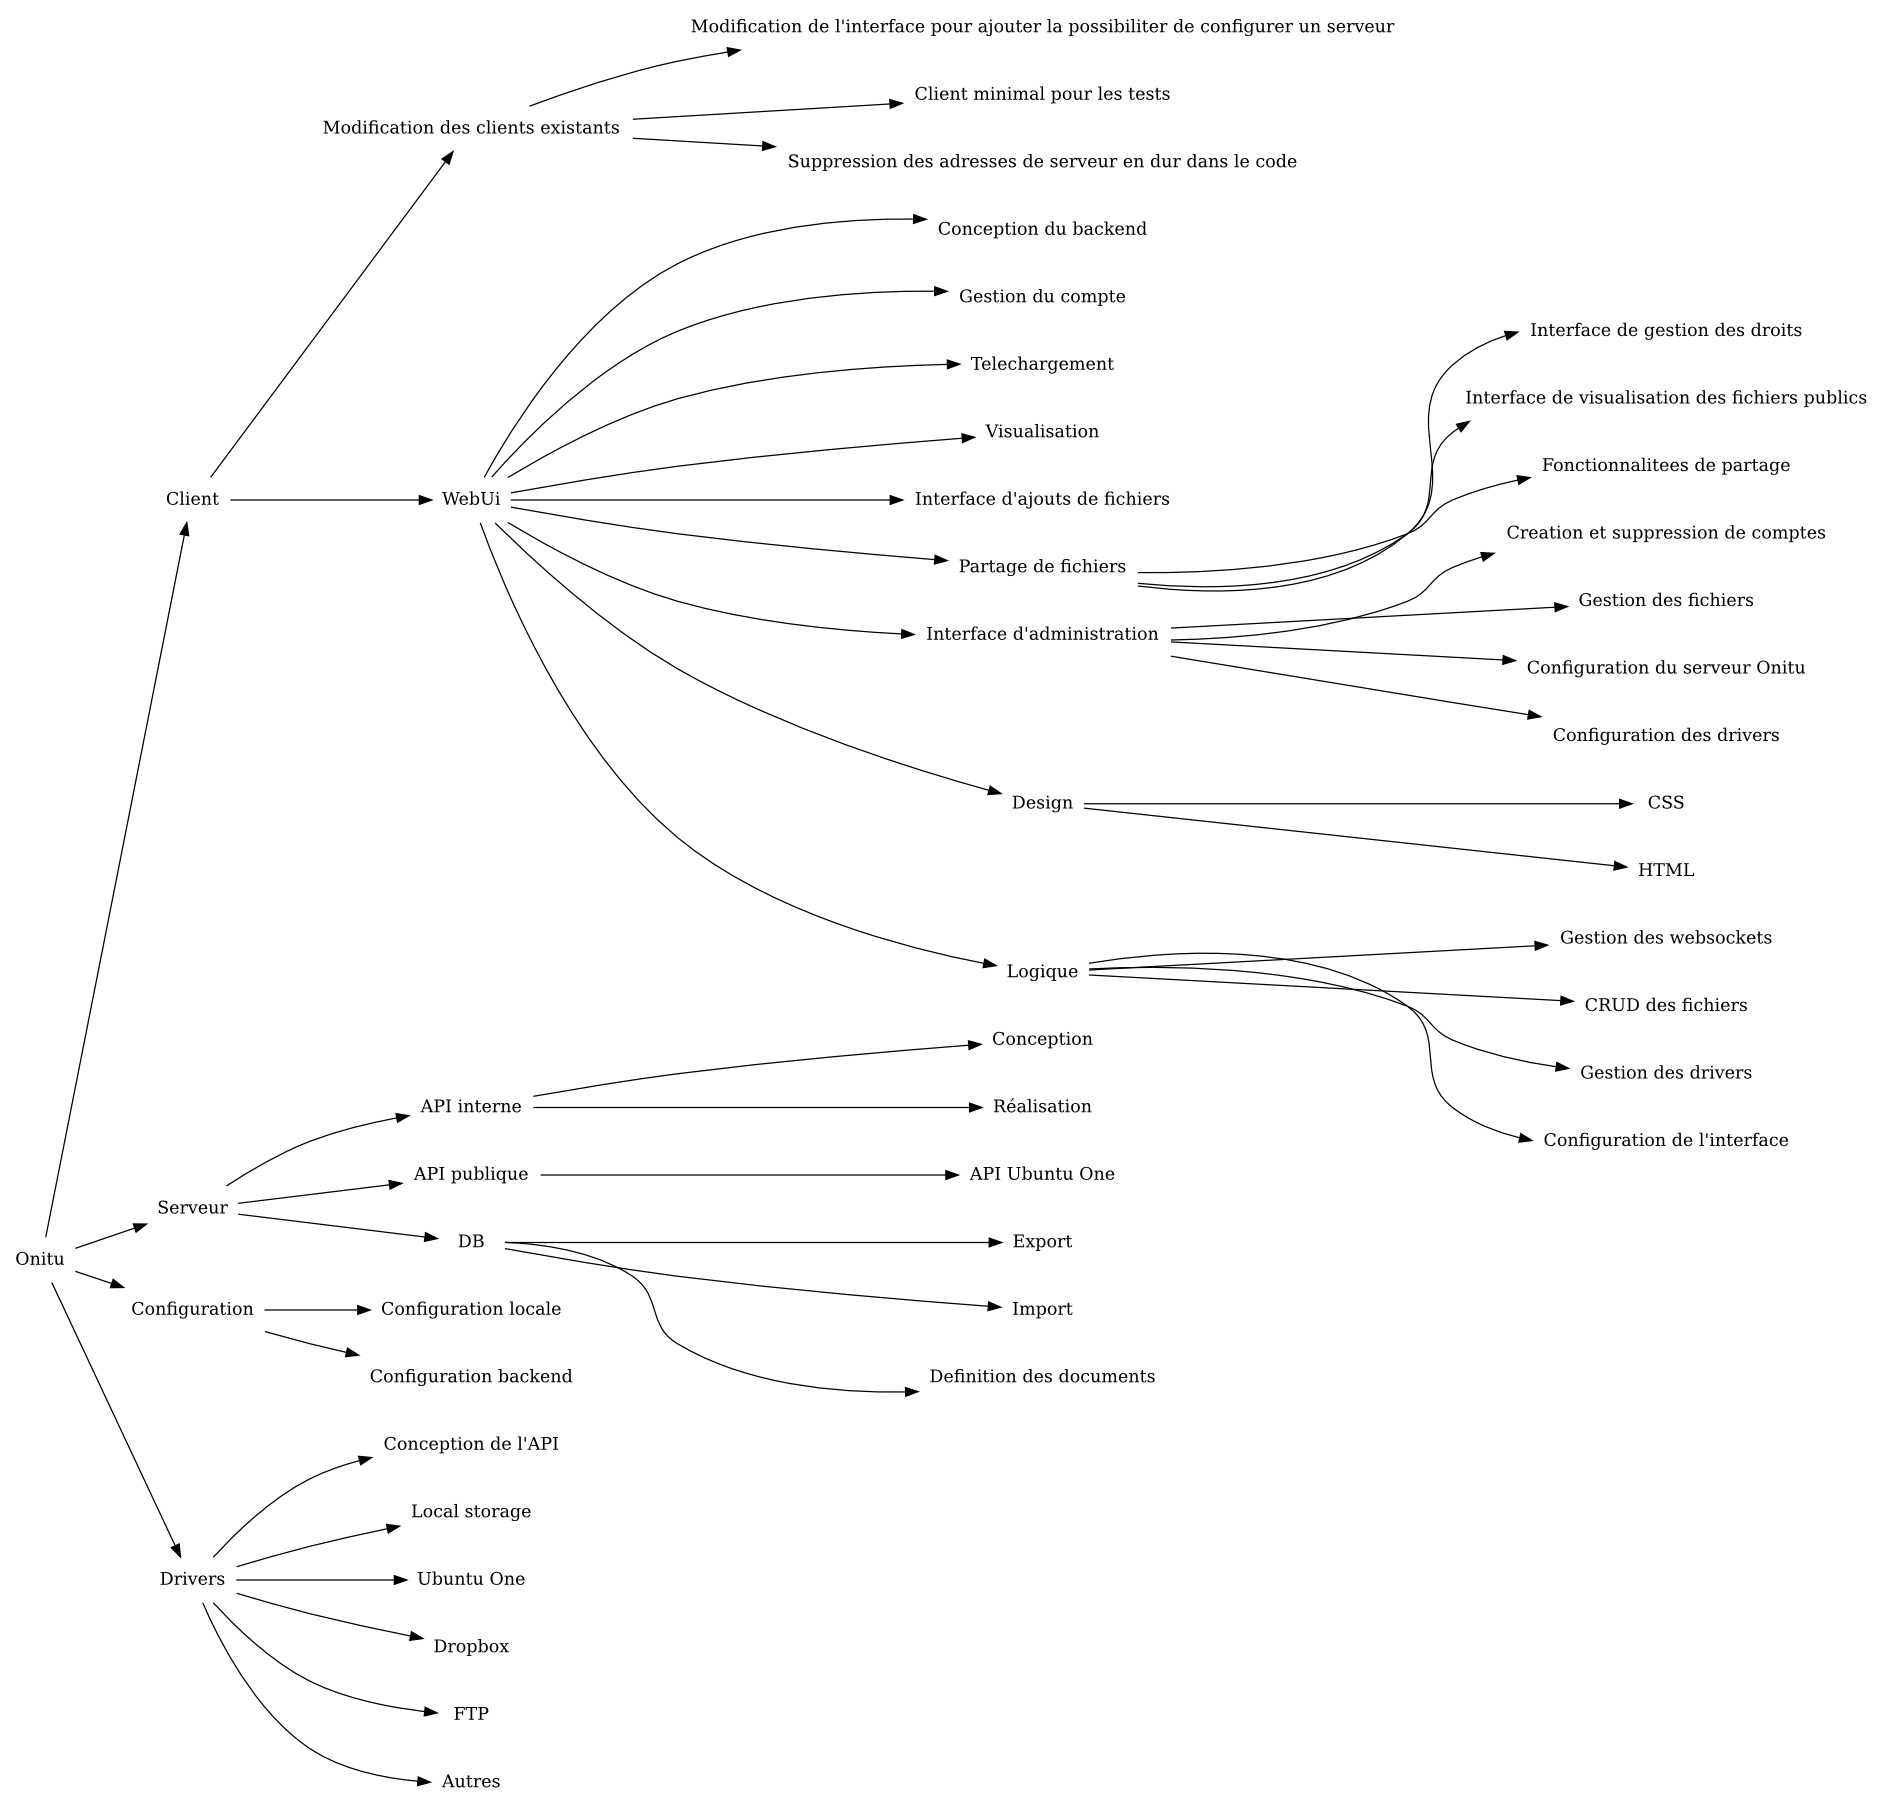
\includegraphics[width=\textwidth,height=\textheight,keepaspectratio]{wbs.png}
    \caption{Work Breakdown Structure}
\end{figure}

\section{Gantt}

\begin{tikzpicture}[y=0.6cm]
  \begin{ganttchart}
    [vgrid,y unit chart=0.5cm, bar height=0.5]{23}
\gantttitle {Gantt Onitu}{23} \\
\gantttitlelist{2013}{8} \gantttitlelist{2014}{12} \gantttitlelist{2015}{3} \\
\gantttitlelist{5,...,12}{1} \gantttitlelist{1,...,12}{1} \gantttitlelist{1, 2, 3}{1}\\
\ganttgroup {LabEIP}{1}{22} \\
\ganttmilestone{Communication}{14}
\ganttmilestone[inline, milestone label inline anchor/.style={left=5pt}]{Plan de promotion exterieure}{14}
\ganttmilestone[inline, milestone label inline anchor/.style={right=5pt}]{Forum eip}{18.5} \\
\ganttmilestone{Bilans}{14.5}
\ganttmilestone[inline, milestone label inline anchor/.style={left=5pt}]{tech final tek4}{14.5}
\ganttmilestone[inline, milestone label inline anchor/.style={left=5pt}]{tech final}{21} \\
\ganttmilestone{Soutenances}{3}
\ganttmilestone[inline, milestone label inline anchor/.style={right=5pt}]{bilan architecture}{3}
\ganttmilestone[inline, milestone label inline anchor/.style={left=5pt}]{finale tek5}{22}
\ganttmilestone[inline, milestone label inline anchor/.style={left=5pt}]{finale tek4}{17} \\
\ganttgroup {Onitu}{1}{21} \\
\ganttgroup {Client}{6}{21} \\
\ganttgroup {Modification clients}{6}{14} \\
\ganttbar {Modification des interfaces }{11}{13}
\ganttbar [inline, bar label inline anchor/.style={left=20pt}]{[Groupe client] 5j/h }{11}{13} \\
\ganttbar {Client minimal pour les tests}{6}{7}
\ganttbar [inline, bar label inline anchor/.style={left=20pt}]{[] j/h }{6}{7} \\
\ganttbar {Suppression des adresses en dur}{13}{14}
\ganttbar [inline, bar label inline anchor/.style={left=20pt}]{[] j/h }{13}{14} \\
\ganttgroup {WebUi}{9}{21} \\
\ganttbar {Conception du backend}{9}{12}
\ganttbar [inline, bar label inline anchor/.style={left=20pt}]{[] j/h }{9}{12} \\
\ganttbar {Gestion du compte}{16}{19}
\ganttbar [inline, bar label inline anchor/.style={left=20pt}]{[] j/h }{16}{19} \\
\ganttbar {Telechargement}{16}{18}
\ganttbar [inline, bar label inline anchor/.style={left=20pt}]{[] j/h }{16}{18} \\
\ganttbar {Visualisation}{21}{21}
\ganttbar [inline, bar label inline anchor/.style={left=20pt}]{[] j/h }{21}{21} \\
\ganttbar {Interface d'ajouts de fichiers}{16}{18}
\ganttbar [inline, bar label inline anchor/.style={left=20pt}]{[] j/h }{16}{18} \\
\ganttgroup {Partage de fichiers}{17}{21} \\
\ganttbar {Gestion des droits}{17}{20}
\ganttbar [inline, bar label inline anchor/.style={left=20pt}]{[] j/h }{17}{20} \\
\ganttbar {Visualisation des fichiers publics}{20}{21}
\ganttbar [inline, bar label inline anchor/.style={left=20pt}]{[] j/h }{20}{21} \\
\ganttbar {Fonctionnalitees de partage}{18}{19}
\ganttbar [inline, bar label inline anchor/.style={left=20pt}]{[] j/h }{18}{19} \\
\ganttgroup {Interface d'administration}{12}{14} \\
\ganttbar {Creation et suppression de comptes}{13}{13}
\ganttbar [inline, bar label inline anchor/.style={left=20pt}]{[] j/h }{13}{13} \\
\ganttbar {Gestion des fichiers}{12}{14}
\ganttbar [inline, bar label inline anchor/.style={left=20pt}]{[] j/h }{12}{14} \\
\ganttbar {Configuration du serveur Onitu}{12}{13}
\ganttbar [inline, bar label inline anchor/.style={left=20pt}]{[] j/h }{12}{13} \\
\ganttbar {Configuration des drivers}{12}{13}
\ganttbar [inline, bar label inline anchor/.style={left=20pt}]{[] j/h }{12}{13} \\
\ganttgroup {Design}{15}{16} \\
\ganttbar {CSS}{15}{16}
\ganttbar [inline, bar label inline anchor/.style={left=20pt}]{[] j/h }{15}{16} \\
\ganttbar {HTML}{15}{16}
\ganttbar [inline, bar label inline anchor/.style={left=20pt}]{[] j/h }{15}{16} \\
\ganttgroup {Logique}{10}{16} \\
\ganttbar {Gestion des websockets}{13}{16}
\ganttbar [inline, bar label inline anchor/.style={left=20pt}]{[] j/h }{13}{16} \\
\ganttbar {CRUD des fichiers}{12}{14}
\ganttbar [inline, bar label inline anchor/.style={left=20pt}]{[] j/h }{12}{14} \\
\ganttbar {Gestion des drivers}{10}{12}
\ganttbar [inline, bar label inline anchor/.style={left=20pt}]{[] j/h }{10}{12} \\
\ganttbar {Configuration de l'interface}{10}{11}
\ganttbar [inline, bar label inline anchor/.style={left=20pt}]{[] j/h }{10}{11} \\
\end{ganttchart}
\end{tikzpicture}

\begin{tikzpicture}[y=0.8cm]
\begin{ganttchart}
    [vgrid,y unit chart=0.7cm, bar height=0.6]{23}
\gantttitle {Gantt Onitu}{23} \\
\gantttitlelist{2013}{8} \gantttitlelist{2014}{12} \gantttitlelist{2015}{3} \\
\gantttitlelist{5,...,12}{1} \gantttitlelist{1,...,12}{1} \gantttitlelist{1, 2, 3}{1}\\
\ganttgroup {LabEIP}{1}{22} \\
\ganttmilestone{Communication}{14}
\ganttmilestone[inline, milestone label inline anchor/.style={left=5pt}]{Plan de promotion exterieure}{14}
\ganttmilestone[inline, milestone label inline anchor/.style={right=5pt}]{Forum eip}{18.5} \\
\ganttmilestone{Bilans}{14.5}
\ganttmilestone[inline, milestone label inline anchor/.style={left=5pt}]{tech final tek4}{14.5}
\ganttmilestone[inline, milestone label inline anchor/.style={left=5pt}]{tech final}{21} \\
\ganttmilestone{Soutenances}{3}
\ganttmilestone[inline, milestone label inline anchor/.style={right=5pt}]{bilan architecture}{3}
\ganttmilestone[inline, milestone label inline anchor/.style={left=5pt}]{finale tek5}{22}
\ganttmilestone[inline, milestone label inline anchor/.style={left=5pt}]{finale tek4}{17} \\
\ganttgroup {Onitu}{1}{21} \\
\ganttgroup {Serveur}{1}{18} \\
\ganttgroup {API interne}{1}{10} \\
\ganttbar {Conception}{1}{8}
\ganttbar [inline, bar label inline anchor/.style={right=20pt}]{[] j/h }{1}{8} \\
\ganttbar {Réalisation}{6}{10}
\ganttbar [inline, bar label inline anchor/.style={right=20pt}]{[] j/h }{6}{10} \\
\ganttgroup {API publique}{6}{10} \\
\ganttbar {API Ubuntu One}{6}{10}
\ganttbar [inline, bar label inline anchor/.style={right=20pt}]{[] j/h }{6}{10} \\
\ganttgroup {DB}{6}{12} \ganttbar {Export}{11}{12} \\
\ganttbar [inline, bar label inline anchor/.style={right=20pt}]{[] j/h }{11}{12} \\
\ganttbar {Import}{11}{12}
\ganttbar [inline, bar label inline anchor/.style={right=20pt}]{[] j/h }{11}{12} \\
\ganttbar {Definition des documents}{6}{7}
\ganttbar [inline, bar label inline anchor/.style={right=20pt}]{[] j/h }{6}{7} \\
\ganttgroup {Configuration}{8}{11} \\
\ganttbar {Configuration locale}{9}{11}
\ganttbar [inline, bar label inline anchor/.style={right=20pt}]{[] j/h }{9}{11} \\
\ganttbar {Configuration backend}{8}{11}
\ganttbar [inline, bar label inline anchor/.style={right=20pt}]{[] j/h }{8}{11} \\
\ganttgroup {Drivers}{1}{18} \\
\ganttbar {Conception de l'API}{1}{7}
\ganttbar [inline, bar label inline anchor/.style={right=20pt}]{[] j/h }{1}{7} \\
\ganttbar {Local storage}{6}{8}
\ganttbar [inline, bar label inline anchor/.style={right=20pt}]{[] j/h }{6}{8} \\
\ganttbar {Ubuntu One}{6}{8}
\ganttbar [inline, bar label inline anchor/.style={right=20pt}]{[] j/h }{6}{8} \\
\ganttbar {Dropbox}{9}{12}
\ganttbar [inline, bar label inline anchor/.style={right=20pt}]{[] j/h }{9}{12} \\
\ganttbar {FTP}{11}{13}
\ganttbar [inline, bar label inline anchor/.style={right=20pt}]{[] j/h }{11}{13} \\
\ganttbar {Autres}{13}{18}
\ganttbar [inline, bar label inline anchor/.style={right=20pt}]{[] j/h }{13}{18} \\
\end{ganttchart}
\end{tikzpicture}


\chapter{Annexes}
\thispagestyle{EIP}

\end{document}
